\documentclass[letterpaper,twocolumn,10pt]{article}

\usepackage[margin=1in]{geometry}
%\usepackage{endnotes,multirow}
\usepackage{refstyle,amsmath,chngcntr}
\usepackage{epsfig,subfigure,framed}
\usepackage{textcomp} % for tilde
\usepackage{paralist} % for in-paragraph lists
\usepackage{parskip} % For making paragraphs split by new lines instead of indents
\usepackage{graphicx}
\usepackage{hyperref}

% Used for changing the spacing after the title, sections, and subsections.
\usepackage{titlesec,titling}

% Used for code snippets
\usepackage{listings,courier}

% Make text in figure captions small
\usepackage{caption3} % load caption package kernel first
%\DeclareCaptionOption{parskip}[]{} % disable "parskip" caption option
\usepackage{caption}

% Make sure that figure numbers are continuous through the document
\counterwithout{figure}{section}
\counterwithout{figure}{subsection}

% Settings on code listings.
\lstset{language=C,
		xleftmargin=0pt,
		xrightmargin=0pt,
		framexbottommargin=0pt,
        framextopmargin=0pt,
        framesep=0pt}

\lstdefinelanguage
   [x64]{Assembler}     % add a "x64" dialect of Assembler
   [x86masm]{Assembler} % based on the "x86masm" dialect
   % with these extra keywords:
   {morekeywords={LOCK,XCHG,CMP,JZ,JNZ,CALL, %
                  rax,rdx,rcx,rbx,rsi,rdi,rsp,rbp, %
                  r8,r8d,r8w,r8b,r9,r9d,r9w,r9b}} % etc.

% Modify spacing before/after title, sections, and subsections.
%\setlength{\droptitle}{-3em}  %--------sigalternate----------
%\posttitle{\par\end{center}\vspace{-1.5em}} %--------sigalternate----------
\newcommand{\Sref}[1]{Section~\ref{#1}} 

% Add a horizontal rule above captions, and make captions closer to their figures
\DeclareCaptionFormat{ruled_caption}{#1#2#3\hrulefill}
\captionsetup[figure]{format=ruled_caption}

% Prevent footnotes from spanning multiple pages
\interfootnotelinepenalty=10000

% For leaving some comments in the draft.
\newcommand{\comment}[1]{}
\newcommand{\TextToolname}{Malcontent}
\newcommand{\Toolname}{\textsc{\TextToolname{}}}
\newcommand{\BoldToolname}{\textsc{\bf\TextToolname{}}}

% For getting rid of copyright box
\makeatletter
\def\@copyrightspace{\relax}
\makeatother

% Modify spacing before the title
\setlength{\droptitle}{-3em} 

\begin{document}

%don't want date printed
\date{}

%make title bold and 14 pt font (Latex default is non-bold, 16 pt)
\title{\Large \bf \Toolname: Cache Line Contention Detection for COTS Binaries}
\author{
{\rm Peter Goodman} \hspace{1.5em} {\rm Angela Demke Brown} \hspace{1.5em} {\rm Ashvin Goel}\\
University of Toronto
} % end author
\maketitle

%\begin{abstract}
%\end{abstract}

\subsection*{Abstract}
Cache-line contention is an increasingly important problem in multi-threaded applications running on cache coherent SMPs.
Contention on cache lines is symptomatic of both performance and correctness bugs. In terms of performance, cache line
contention limits scalability by introducing extra latency when accessing shared memory.  In terms of correctness, cache
line contention can also be caused by data races, which introduce non-determinism into one's program.

In this paper, we describe \Toolname, a system that detects and diagnoses cache line contention in arbitrary binary programs.
\Toolname{} refines existing contention detection approaches in several novel ways. First, we describe a method training
a detection system to focus on only the code and data that matter to the problem. Second, we describe a new form of
data-centric sampling: comprehensive data sampling. Our sampling approach uses unlimited watchpoints to uniformly
sample memory locations according to the type of data stored in memory. This avoids sampling bias where a large portion
of a program's memory is unshared.

\section{Introduction}\label{sec:intro}

In multi-threaded applications, cache-line contention is a symptom of several kinds of bugs: data races, true sharing,
false sharing, and pseudo sharing. Data races are potential correctness bugs that introduce non-determinism into running
programs. True, false, and pseudo sharing are performance bugs that limit the scalability of multi-threaded applications
\cite{ImpactOfFalseSharing}. Both problems are important in the multi-core era, where the level of concurrency in
applications is growing to match the additional processing power provided by increasing core counts on modern processors.

% Despite this rise in importance, detecting and diagnosing false
%sharing in large systems remains challenging. Due to the nature of cache coherent multiprocessors, false
%sharing is often indistinguishable from true sharing (including data races). Also, diagnosing the cause
%of false sharing requires that one distinguish accesses to the same objects from ``pseudo sharing", which
%occurs when two nearby objects are separately but concurrently accessed \cite{DegenerateSharingAndFalseCoherence}.

This paper presents \BoldToolname{}, a software-only runtime for precisely detecting and diagnosting cache line
contention in commercial, off-the-shelf (COTS) x86-64 program binaries. \Toolname{} addresses three limitations of prior
work: \begin{enumerate}
\item They are not general: they require an understanding of the semantics of all synchronization primitives used
by the program. This is unsatisfactory for COTS binaries that employ lock-free algorithms and home-grown synchronization
primitives.

\item They are imprecise: they cannot distinguish between data races, true sharing, false sharing, and pseudo sharing
\cite{DegenerateSharingAndFalseCoherence}. This can result in high false-positive rates or confusing reports that decrease
the usefulness of these tools for practitioners.

\item They are not comprehensive: they miss actual cases of cache line contention because they use heuristics to sample 
or instrument only a subset of the code, and therefore lose visibility on accesses to data that might cause bugs.

%\item They are not selective. While apparently at odds with comprehensiveness, they track or instrument \emph{too much}, 
%and therefore waste time looking for problems where none exist.

%\item They introduce extra cache coherency traffic, which limits scalability and hides performance
%problems. The extra traffic introduced comes from the mechanisms used to track cache line ownership.

%\item They are unable to selectively detect false sharing on only specific types of objects or specific
%code.

\end{enumerate}

\Toolname{} uses dynamic binary translation (DBT) to instrument a program binary and detect cache line contention
at runtime. Our approach combines unlimited watchpoints \cite{UnlimitedWatchpoints,DynamoRIOWatchpoints}, data
sampling, and a lightweight cache line ownership tracking mechanism to detect cache line contention. The key insight
of our approach is that if we know \begin{inparaenum}[i)]
\item what types of data are accessed by more than one thread, and
\item what types of data are accessed by what code, then
\end{inparaenum}
we can efficiently detect cache line contention by selectively instrumenting only the code and the data that matters.

%we can extend on and improve existing techniques to detecting
%cache line contention by combining solutions the following problems:
%\begin{enumerate}
%\item Code concurrency: Detecting what code is executed by more than one thread.
%\item Data concurrency: Detecting what types of data are accessed by more than one thread.
%\item Code polymorphism: Detecting what code accesses what types of data.
%\end{enumerate}

% infinite software watchpoints, as implemented within a DBT system, as
%well as being selective about what parts of the program to 

%The key insight of our
%approach is that accesses to shadow memory can be used as a proxy for accesses to actual memory. By 
%detecting contention on proxied accesses, we can establish beliefs about what code causes false sharing. These
%beliefs are strenghtened and eventually verified by specializing code to proxy memory accesses at increasingly
%finer granularities.

% --------------------------------------
\subsection{Contributions}
This paper makes the following significant contributions:
\begin{itemize}
\item It describes \Toolname{}, a software-only system that dynamically and precisely diagnoses cache line
contention in multi-threaded, COTS binaries. This enables \Toolname{} to detect performance
and correctness bugs in programs using home-grown synchronization primitives and lock-free algorithms.

\item It describes a new data-centric sampling approach, \emph{comprehensive data sampling}, that improves
sampling coverage and contention detection accuracy. Comprehensive sampling uniformly samples objects in
memory  according to their type. This avoids problems related to sampling bias in situations where a
relatively small amount of shared data is crowded out by a much larger amount of unshared data (as happens
when multi-threaded programs operate on partitions of a data set).

%from wasting cycles looking for contention on
%unshared data
%This is beneficial because it improves coverage: if 90\% of false sharing occurs because of accesses
%to only 10\% of the data, then \Toolname{} will not miss those races by blindly focusing on the other 90\% of data

\item It describes a novel separation of cache line contention detection into two phases:

1. {\bf Training:} an ahead-of-time, heavyweight analysis of the program's execution that
discovers what code can contain cache line contention, and what data is shared by multiple threads. A key
aspect of this phase is that it \emph{does not} need to exhibit any cache line contention; the only requirement
is that training and production workloads exercise/cover the code in similar ways.

% TODO: Evaluate by showing the percentage of code that doesn't get instrumented at all, or is only
% instrumented with lightweight instrumentation.

2. {\bf Detection:} an online analysis that detects cache line contention by selectively
instrumenting only the relevant code and sampling only the relevant data as recognized by the
offline training phase.

This separation is motivated by the need to reduce instrumentation overheads of the detection phase by
as much as possible in order to maximize the detection accuracy (e.g. data races are time-sensitive). The key
insight enabling this separation is that time--and therefore the cost of instrumentation--does not matter to
the accuracy of the results produced by the training phase.

%A key aspect of the training phase is that it must exhibit approximately the same code coverage as a
%production
%that it does not need to exhibit a buggy execution (i.e. contain actual
%cache line contention)

%It describes a novel separation of cache line contention detection into two phases: \begin{enumerate}
%\item[1) \emph{Training:}] This phase uses heavyweight instrumentation to discover \begin{inparaenum}
%\item what code is hot;
%\item what code is executed by more than one thread;
%\item what code accesses what data; and,
%\item function call graphs.
%\end{inparaenum}
%
%This information enables the detection phase to selectively prune the set of code that is instrumented,
%and the set of data that is sampled in order to reduce overheads. 
%
%\item[2) \emph{Detection:}] 
%\end{enumerate}

%ahead-of-time training phase that discovers code and data that can be ignored
%during online analysis, thus reducing online instrumentation overheads. The key insight is that all training
%data gathered is 
%time--and
%time spent--doing offline analysis does not affect the accuracy of the results produced. This is important
%because discovering what code can be pruned and what data does

%the detection of what code should be instrumented and what data should be sampled is \emph{not} time-sensitive, and
%therefore can be performed any time. 
%
%using results gathered from an offline learning and analysis phase. This separation is motivated by recognizing that 

%\item It presents two new techniques, \emph{proxy memory} and \emph{tagged reads}, that enable
%efficient determination of memory access behavior using shadow memory. Unlike existing shadow
%memory systems, proxy memory is not treated as a mutable meta-data store. This avoids extra
%serialization and coherence traffic introduced by prior work when dynamically manipulating shadow state.

%\item It describes two new, data-centric sampling approaches: uniform heap sampling, and selective heap
%sampling. .
%Once data of interesting has been narrowed down, \Toolname{} can apply selective heap sampling, which
%focuses sampling on specific types of objects or data accessed by specific code (or both).
\end{itemize}

% TODO: Define precise
% TODO: Define false-sharing

% --------------------------------------------------------------------------------------

\section{Overview}\label{sec:overview}

\Toolname{} uses the Granary DBT \cite{Granary} framework to instrument the memory accesses of a program while
it is running. During the offline training phase, DBT is used to figure out what data is accessed by more than one thread,
and what code accesses that data. During its online detection phase, \Toolname{} uses Granary's implementation of unlimited
watchpoints to watch for accesses to a representative sample of cache lines, assign owning threads to those cache lines,
and finally detect transfers in ownership.

\subsection{Definitions}
\Toolname{} looks for cache line contention bugs of the following forms:

{\bf Data races} occur when the same program variable is concurrently modified by two threads, or 
modified by one thread and concurrently accessed by another thread, and where neither access is atomic (e.g. using
and atomic read-modify-write instruction).

{\bf True sharing} has the same access pattern as a data race, except that one or both operations
are atomic.

{\bf False sharing} occurs when two semantically related variables (e.g. two fields in a struct) occupy
the same cache line and are concurrently accessed, thus introducing contention on the cache line.

{\bf Pseudo sharing} occurs when two semantically unrelated variables (e.g. fields in adjacent structs,
adjacent array entries) occupy the same cache line and are concurrently accessed \cite{DegenerateSharingAndFalseCoherence}.

% --------------------------------------
\subsection{Mechanisms}

% --------------------------------------
\paragraph{Training}
%\paragraph{Code Concurrency Analysis }
%\Toolname{} analyzes code to determine what code is executed by more than one thread. This analysis allows \Toolname{}
%to either not instrument, or only very lightly instrument, non-concurrent code during its detection phase. The insight is
%that code that does get executed by more than one thread is more likely to operate on shared data than code that is
%only ever observed (during training) to have been executed by a single thread.
%
%There are some important cases where this insight does not hold. For example, in a single writer, multiple reader queue,
%the code implementing writes to the queue might only be executed by a designated writer thread, and therefore never
%be marked as concurrent. Obviously, there is contention bet

%\paragraph{Data Concurrency Analysis}
\Toolname's training phase focuses on reducing detection overheads by finding code that doesn't need to be instrumented
during the detection phase. The key challenge of this phase is determining what code can safely be pruned without negatively
affecting the accuracy of the detection phase. Our insight is that the detection phase should only look for cache contention
on accesses to shared data structures. To do this, we must know \begin{inparaenum}
\item what data structures are shared, and
\item what code accesses those data structures.
\end{inparaenum}

\newcommand\TypeId{$TypeID$}
\newcommand\TypeIdPair{$\langle PC,size \rangle$ }

We implemented these analyses using Granary's address watchpoints \cite{AddressWatchpoints} system, which allows us to
``taint" addresses and then interpose on instructions using tainted addresses to access memory. Using Granary, we interpose on
all dynamic memory allocator functions and taint every address returned by those functions with an abstract \TypeId{}.
Each \TypeId{} uniquely identifies an allocation context in terms of a \TypeIdPair{} pair, where $PC$ is the program counter
to which the allocation function will return, and $size$ is the number of bytes being allocated. This arrangement allows us to
approximate the actual number of distinct types of program data structures for arbitrary binaries, even in the absence of
static source code information or debug information.

We use per-type shadow memory to detect data structure sharing accross multiple threads.
We associate each \TypeId{} with a small amount of shadow memory: $\langle InitialThreadId,\linebreak[0]IsShared \rangle$. This
arrangement means that every allocated address tainted by the same \TypeId{} is indirectly associated with the same
shadow memory. If this is the first allocation for a \TypeId, then the shadow memory is initialized to
$\langle CurrThreadId,\linebreak[0]false \rangle$. Sharing is detected and marked either by subsequent allocations for the
same \TypeId{} but by different threads than the initial thread, or by accesses to tainted addresses by threads other
than the initial thread.

To detect what code accesses what types of data, we propagate the {\TypeId}s to code on every memory access to
a tainted address. Finally, to determine what code accesses shared data, we combine the output of both analyses to
produce, for each basic block of code executed during training, we report on whether or not it contained accesses
to shared data structures. During the detection phase, we heavily instrument only those blocks that contain accesses
to shared data structures, or (to be conservative) were never executed during the training phase.

%taint from the address to the code accessing the memory associated with tainted address.
%This allows us to identify what code is accessing what types of data.
%Later allocations do not modify the shadow, unless the thread performing the
%allocation does not 
%When an
%object is allocated, its address is tainted with \TypeId, and, if this is a new \TypeId, then the sha
%and which is initialized 
%Every time a tainted address is accessed, we perform the following: \begin{enumerate}
%\item Propagate 
%
%\item Check if the current thread matches the $AllocThread$. If not, then set $IsShared \gets true$. Future accesses to an
%object with $IsShared = true$ d
%
%\end{enumerate}
% identifier that is
%uniquely associated with the allocation context 
%associated with the allocation context, as represented by a \TypeIdPair{} pair.
%For each dynamically allocated data structure, we ``taint'' the address of the 
%Pruning code 
%This analysis determines what types of data are shared, i.e. accessed by more than one thread, so that the 
%\Toolname{}'s training phase analysis data access patterns to determine what types of data are accessed by more than one
%thread. The insight is that we should only look
%\paragraph{Code Polymorphism Analysis}

% --------------------------------------
\paragraph{Detection}

The detection phase is composed of three components: 

1. {\bf The interposition layer}. We interpose on dynamic memory allocators and record the most recently allocated
address for each \TypeId{}. The set of all most recently allocated objects forms the population of addresses from which
we sample.

As a minor optimization, we restrict ourselves to only those {\TypeId}s associated that were found during training
to be associated with shared data structures. Also, unlike during the training phase, we \emph{do not} taint any
addresses.

2.  {\bf The monitor}. The monitor is a separate thread, spawned by \Toolname{} at program startup, and is responsible
for implementing \Toolname's \emph{comprehensive data sampling}. The monitor thread periodically
wakes up, chooses a sample set using a round-robin algorithm over the population of recently allocated addresses by type, and
then enables software watchpoints on all sampled addresses.

After enabling the watchpoints, the monitor goes to sleep. When it next wakes up, it removes any active watchpoints
and generates reports on any cache line contention that was detected. Finally, it restarts the sampling process.

3. {\bf The instrumentation}. There are two tiers of instrumentation: lightweight and heavyweight. Lightweight
instrumentation applies to all basic blocks of code identified during training as \emph{not} containing accesses to shared
data. Lightweight instrumentation exists to maintain Granary's control over the program binary, and therefore to maintain
the comprehensiveness of the analysis.

The heavyweight instrumentation implements a form of ``unlimited watchpoints" \cite{UnlimitedWatchpoints}. The
granularity of each watchpoint is a cache line, but can easily be adjusted in order to model systems with smaller or
larger cache line sizes\footnote{The granularity of shadow memory is tunable via a command-line argument}.
In our setup, every 64 bytes of memory has its own shadow memory and watchpoint. Note that
this does not model actual hardware limits on cache sizes and cache contention caused by associativity.

When a memory address is accessed, the instrumentation checks the shadow memory to see if the watchpoint for
the current address is set. If it is, then the instrumentation code further checks to shadow to see if another thread
owns the cache line (in which case contention is detected), or if the current thread can take ownership of the cache line.

% --------------------------------------------------------------------------------------

\section{Related Work}\label{sec:background}
\Toolname{} draws on and extends/refines techniques from existing race detectors and false sharing detectors.

%% --------------------------------------
\paragraph{Dr. Memory}
Dr. Memory \cite{DrContention} implements a set of tools for detecting cache line contention, thread correlations,
and true/false sharing detection in COTS binary programs. Dr. Memory uses the DynamoRIO \cite{DynamoRIO} DBT system
and the Umbra shadow memory framework \cite{Umbra} to interpose on memory accesses and implement their
detection tools. Dr. Memory's contention tool implements the following algorithm for detecting contention. Before each
memory write,  instrumentation performs a ``racy" check to see if the current thread owns the cache line being accessed.
If the cache line is owned by another thread, then a report is generated, and ownership is transferred. If the cache line is
unowned, then ownership is established.

This approach has two drawbacks. First, every time ownership is transferred/established, there is an additional
memory write, which itself introduces CPU overheads due to contention on the cache lines of the shadow memory. Second,
ownership is tracked on data that is never shared. This introduces extra CPU and memory overheads by instrumenting
too much code and tracking too much data.

\Toolname{} addresses both problems. First, its offline learning phase prunes the set of code that should be instrumented.
This has the side effect of reducing the physical memory requirements of shadow memory because fewer instructions will
introduce shadow accesses, and therefore less shadow is accessed. Second, our sampling approach means that ownership
is only tracked for ``watched" objects. This introduces an additional racy read at the beginning of instrumentation, but the
benefit is that the majority of shadow accesses are read-only, and therefore do not generate as much additional contention
on the cache lines associated with shadow memory.

%% --------------------------------------
\paragraph{DataCollider}
DataCollider \cite{DataCollider} is a precise, sampling-basbased oned race detector for the WIndows kernel. DataCollider's key
novelties are its extremely low overhead, as well as its generality: it detects data races without any understanding of
a system's underlying synchronization primitives. DataCollider uniformly samples code by introducing breakpoints into the code.
When a breakpoint is hit, a hardware watchpoint is added to data that was about to be accessed by the interrupted instruction.
Then, the interrupted thread is paused for a short period of time to give another thread the opportunity to access the
same data. If the data is accessed by a second thread while the first thread is paused, then the watchpoint will detect the
access, thus allowing DataCollider to detect a race ``in the act."" 

While this approach is elegant in its simplicity, it has two major drawbacks. First, its dependence on hardware watchpoints
limits it to being able to detect races on at most four distinct 8-byte memory locations simultaneously \cite{IntelSDManual}.
Second, in some cases, it cannot be generalized to detecting arbitrary cache contention when the one contending access
\emph{happens-before} the other \cite{VectorClocks}. For example, if true/false sharing frequently occurs within critical sections;
however, this would be missed by a naiive generalization of the DataCollider algorithm to this problem.

%% --------------------------------------
%\paragraph{Predator}

% TODO: I should really write about this, but time :-(

%% --------------------------------------
\paragraph{Other}

%Intel's VTune \cite{IntelVTune} an an imprecise, sampling-based profiler that can detect false sharing using hardware performance
%counters and monitoring events. It provides detailed, architecture-specific performance-tuning suggestions. Unlike \Toolname{},
%VTune can only report individual program counters that general cache coherency events, but cannot correlate threads by showing
%two contending stack traces.

%, thus triggering the watchpoint and detecting a race ``in the act".
%
%%sampling based approach enables it to be general
%
% The key strengths of
%DataCollider is that it has low overhead, it is independent of the synchronization mechanisms being employed, and that
%it often catches both threads in the act.  This brilliantly simple approach was the main inspiration
%for \Toolname{}. \Toolname{} differs from DataCollider, in that the latter is code-centric insofar as it samples code, whereas
%\Toolname{} is data-centric insofar as it samples data.

%In either case, a memory write occurs to take ownership.

%\DrContention{} comprehensively interposes on
%all memory accesses to track ownership of all cache lines. Every instruction is instrumented to first check if the current
%thread owns the cache line. If not, then the thread is added to the cache line's \emph{threadset}. 

% TODO: Evaluate by disabling is_watched check, i.e. perform ownership tracking on all cache lines, vs. only a subset
% of cache lines.

%Several tracking mechanisms are discussed, including ones that
%track strict ownership transers, and others that attempt to measure thread correlations and the impact of of cache line
%invalidations. The drawback of this approach is that it necessitates checking and updating the shadow memory on every
%memory access, which introduces performance overhead due to extra cache line contention.

%Like \DrContention{}, \Toolname{} uses DBT and shadow memory to track ownership of cache lines. However, \Toolname{}
%only tracks cache line ownership for a subset of the cache lines (those currently being sampled). This makes a big difference
%because, although potentiall all instructions are instrumented for shadow memory, only a small subset of th

Plastic \cite{Plastic} is a Xen-based dynamic false sharing detector and repairer. Plastic uses hardware performance counters
to detect when cache line eviction events due to contention exceed some threshold, and then turns on page-granularity
ownership tracking using hardware page protection. When Plastic discovers sharing of a page, it turns on heavyweight recording
of memory access instructions. Later, it analyzes this record to determine what--if any--cache lines on the page had contention,
and then uses a limited form of DBT to ``patch" the virtualized execution so as to remap previously contended accesses into
non-contending accesses. Plastic's dependence on virtualization limit its ability to find false sharing in arbitrary, binary device
drivers that cannot be virtualized.

%
%SHERIFF \cite{SHERIFF} is a precise false-sharing detector and repairer that works in a similar way to Plastic. Instead of
%tracking page ownership at the VMM level, it tracks page ownership on a per-application basis by turning threads into
%processes, thus allowing it to bootstrap off of existing OS-provided process memory isolation. SHERIFF detects contention
%using twinning and diffing of shared pages \cite{TreadMarks}, and fixes false-sharing using a combination of delaying and 

Eraser \cite{Eraser} is a dynamic race detector that uses shadow memory to track the set of locks that must be held in order
to access shared data. Eraser initially associates the set of all locks with every shared variable. As shared variables are accessed,
their lock sets are refined based on observing the current set of locks held by a particular thread. If a shared variable's lockset
is refined to the empty set, then a data race has potentially been discovered. The benefit of this approach is that it has the
ability to predict data races, even if two accesses were never truly concurrent. The drawback is that a lockset approach is
challenging to generalize: it requires a complete understanding of a program's locking discipline.

Other work based on Lamport's \emph{happens-before} relationship \cite{VectorClocks} can precisely distinguish data races
from true sharing by recognizing that synchronizing operations (such as locks and condition variables) introduce a strict ordering of
accesses. Under this lens, true sharing occurs when two threads access the same variable, but where one of the accesses happens-%
before the other due to the presence of a synchronizing operation. A data race occurs where neither operation logically happens-%
before the other. Like Eraser, generalizing happens-before to arbitrary COTS binaries can be challenging as it requires an
understanding of the sycnrhonization primitives used by a program.


%Initially,
%it applies read-only hardware page protection to all shared memory. Then, as threads attempt to write to protected pages, those
%pages are privately mapped as read/write. When the same page is privately mapped by two or more threads, SHERIFF applies
%the twinning and diffing approach of TreadMarks  to detect local changes to shared pages and narrow down
%on instances of false sharing. Like \Toolname{}, SHERIFF uses a coarse-grained mechanism to hint at the potential for races.

%
%Like \Toolname{}, it takes a pipeline-based
%approach that successively narrows down on the root causes of false sharing. Plastic also uses DBT as part of its
%repair mechanism. Plastic's pipeline begins by using hardware performance counters related to cache contention
%events to detect the presence of false-sharing. Then, it applies a similar technique to MultiRace \cite{MultiRace}, in
%that it tracks the dominant access pattern by each thread to memory on a shared page. This information informs
%their repair mechanism, which transparently re-maps memory accesses at a byte granularity.

%
%SHERIFF \cite{SHERIFF} is a false-sharing detector and repairer that works in a similar way to MultiRace and Plastic. Initially,
%it applies read-only hardware page protection to all shared memory. Then, as threads attempt to write to protected pages, those
%pages are privately mapped as read/write. When the same page is privately mapped by two or more threads, SHERIFF applies
%the twinning and diffing approach of TreadMarks \cite{TreadMarks} to detect local changes to shared pages and narrow down
%on instances of false sharing. Like \Toolname{}, SHERIFF uses a coarse-grained mechanism to hint at the potential for races.


%% --------------------------------------
%\subsection{Race Detection}
%
%Race detectors can be categorized according to the following parameters:
%\begin{description}
%\item[Approach] Static or dynamic. \hfill \\
%Static race detectors analyze source code or binaries, typically performing interprocedural control-
%and data-flow analyses. The benefit of static analysis is that they can inspect all program paths.
%
%Dynamic race detectors monitor memory accesses for races. The benefit of this approach is that
%races can be caught "in the act". The drawbacks of this approach is that most dynamic race detectors
%are too slow to run in production environments, and therefore must be tested on simulated workloads.
%If these workloads do not exercise all code paths than many races can be missed. Dynamic race detectors
%can be further broken down into on-the-fly detectors or post-mortem detectors, which analyze memory
%access logs.
%
%\item[Model] Precise or imprecise.  \hfill \\
%Precise race detectors report no false-positives and are usually implemented using Lamport's
%happens-before relationship \cite{VectorClocks}. Precise race detectors often trade efficiency
%for completeness in order to achieve their precision. That is, they sometime miss true races in
%code.
%
%Imprecise race detectors can have high false positive rates, but tend to be more complete in terms of
%including races not detected by precise detectors. They tend to be implemented using a variant of the
%lockset algorithm \cite{Eraser}.
%
%\item[Granularity] Fine-grained or coarse-grained. \hfill \\
%Fine-grained race detectors operate at or close to the granularity of memory accesses. Coarse-grained
%race detectors operate at an object granularity, or at a fixed granularity (e.g. cache line, page).
%
%The granularity of a race detector can affect its precision. For example, a happens-before race detector 
%can be imprecise (i.e. report false positives) by operating at a coarse granularity. If the granularity were
%the size of a cache line, then the race detector would be a cache line contention detector: it would hint
%at races as well as false-sharing.
%
%\item[Mode] Comprehensive or sampling-based. \hfill \\
%Comprehensive race detectors typically analyze every memory read and write. They are usually implemented
%by instrumenting all program code.
%
%Sampling-based race detectors analyze either a subset of the code or a subset of the data. In the former
%case, they focus on detecting races by specific code.
%\end{description}

%Under this categorization scheme, \Toolname{} is a dynamic, precise, variable-granularity, mixed-mode
%false-sharing detector. It draws inspiration from a number of existing race detectors, including LiteRace
%\cite{LiteRace}, MultiRace \cite{MultiRace}, RaceMob \cite{RaceMob}, RaceTrack \cite{RaceTrack}, and
%DataCollider \cite{DataCollider}.
%
%LiteRace \cite{LiteRace} is a precise, sampling-based dynamic race detector implemented on top of the Microsoft
%Pheonix binary translator. It samples at a function granularity, and executes either one specialized version of the
%code or another. The sampling rate for a function is inversely proportional to how often it executes. This is based
%on the insight that races are likely to occur in infrequently executed code, because otherwise they are benign or
%would have been noticed and resolved. This insight, called the ``cold code hypothesis", motivated \Toolname's
%post-mortem ranking scheme: cases of false sharing are more highly ranked when one---but \emph{not} both---of
%the participating threads are executing cold code. This variant on the cold code hypothesis emphasizes the similarly
%hard-to-find case of cold code pessimizing hot code.

%
%MultiRace \cite{MultiRace} is a comprehensive, dynamic race detector that employs a hybrid happens-before and
%lockset-based approach. It operates at an object granularity, and therefore reports false-positives. It is unique
%in that it uses ``pointer swizzing" as a means of remapping memory to ``minipages" that track the dominating
%access pattern of a thread (read-write > read-only > no-access). \Toolname{} uses a similar pointer swizzing approach, but
%in the form of address watchpoints \cite{AddressWatchpoints}. Pointers to heap-allocated objects are ``swizzled" to
%include a type identifier that is unique to a \TypeIdPair{} pair. This improves the diagnosis of false-sharing,
%because it allows \Toolname{} to distinguish between two threads accessing different fields of the same object, and
%two threads accessing two nearby objects of the same (or different) types.
%
%RaceMob \cite{RaceMob} and RaceTrack \cite{RaceTrack} are two hybrid happens-before and lockset-based race detectors.
%RaceMob begins by statically analyzing source code to find potential races (lockset), then dynamically verifies those races
%(happens-before). RaceTrack is a JIT-based race-detector for Microsoft's common language runtime (CLR). It uses the
%concept of threadsets to efficiently maintain happens-before relationships for memory locations and detect the possible
%presence of a race and uses lockets to confirm predicted races. The novelty of RaceTrack is that it adapts the detection
%granularity from object-granularity to field-granularity. \Toolname{} follows the same high-level approach as both RaceMob
%and RaceTrack in that it attempts to predict the source of false-sharing at one granularity, then verify those predictions 
%at another granularity.

%% --------------------------------------
%\subsection{False Sharing Detection}
%
%Similar to race detectors, false-sharing detectors can be sampling-based or comprehensive. Comprehensive approaches
%can be categorized  into simulation-based and instrumentation-based approaches. Simulation-based approaches focus on
%simulating the full cache hierarchy and can distinguish fine-grained events like false sharing due to set-associativity and
%false sharing due to different data being accessed on the same cache line. Instrumentation-based approaches focus more
%on mechanisms for estimating or detecting cache line contention.

%\paragraph{Sampling-based}
%\paragraph{Comprehensive}

% Simulation based approaches:
% TODO: Callgrind/Cachegrind?
% TODO: Simics?
% TODO: Pluto?

% --------------------------------------------------------------------------------------
\section{Methodology}\label{sec:methodology}

\Toolname{} can be thought of as combining DataCollider's sampling based approach \cite{DataCollider}, and Dr. Memory's
cache line ownership tracking approach \cite{DrContention}. The major distinction between \Toolname, DataCollider, and
Dr. Memory are that:
\begin{itemize}
\item \Toolname's sampling approach is data-centric, as opposed to DataCollider's, which is code-centric. That is, DataCollider
interposes on code first in order to find data that should be watched. \Toolname{} starts with the data that it expects to
be shared (based on training), and then waits for code to access that data.

\item Unlike Dr. Memory, \Toolname{} does not heavily instrument all code for cache line ownership tracking, nor does it
persistently track the ownership of all cache lines. Instead, the training phase informs the detection phase on what
instructions to instrument, and sampling turns on temporary tracking of a subset of cache lines. When the \emph{first}
instance of contention is detected, then the issue is reported and tracking is disabled.
\end{itemize}

% --------------------------------------
\subsection{Ownership Tracking}
\begin{figure}
\begin{center}
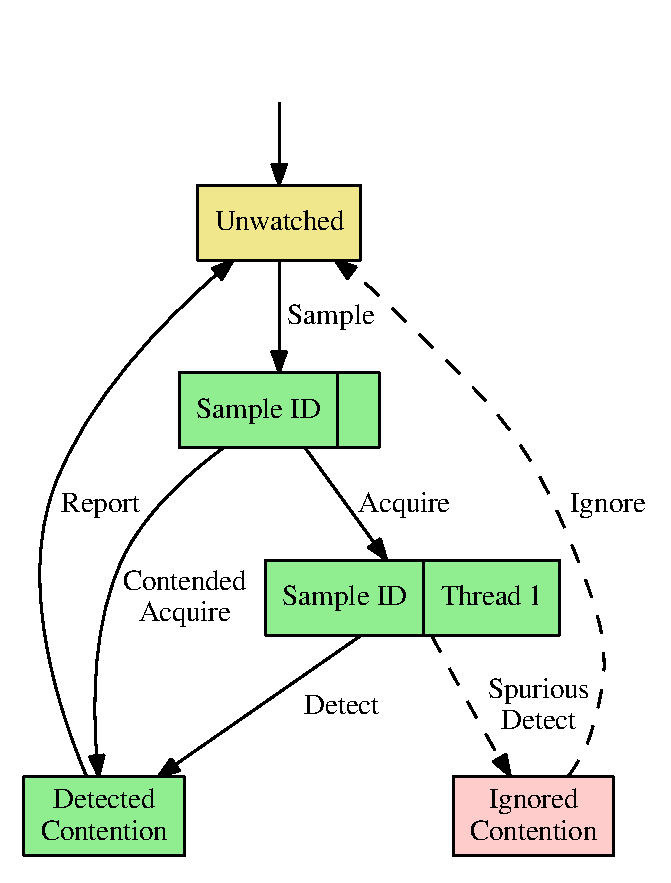
\epsfig{file=states.eps, height=30em}
\end{center}
\caption{\label{fig:states_of_shadow}States of individual shadow memory cells. Each cell tracks the watched and ownership %
status of a cache line. Yellow states are unwatched. Green states are watched. Red states represent contention that was missed %
due to races in the instrumentation. Transitions between states are based on (potentially stale) observed prior states. For %
example, the spurious acquire transition is possible because the decision to make the transition is based on a racy \texttt{CMP} %
against the $SampleId$ (\figref{inline_assembly}). If two threads simultaneously see that the cache line it watched but not %
owned, then both will execute the atomic \texttt{XCHG}, and only one thread will ``win". The ignore transition is induced, %
either because the sampling timeout expires, or more likely, because the report transition occurs.}
\end{figure}

\begin{figure}
\lstset{language=[x64]Assembler}
\begin{lstlisting}[basicstyle=\footnotesize\ttfamily]
;; Racy watchpoint check.
CMP [ShadowAddr + Offs(SampleId)], 0
JZ ignore
;; Racy ownership check.
CMP [ShadowAddr + Offs(ThreadId)], CurrThreadId
JZ ignore
;; Take ownership, or transfer ownership
LOCK XCHG [ShadowAddr], OldState
CALL CheckContention(OldState,Addr,PC)
ignore:
\end{lstlisting}
\caption{\label{fig:inline_assembly}Instrumentation instructions injected for each shared memory access. The algorithm optimizes on %
instruction footprint by using a single \texttt{XCHG} instruction to perform multiple state transitions from %
\Figref{states_of_shadow}, and then figuring out what state we should be in based on the value of $OldState$.}
\end{figure}

Initially, a every cache line is unwatched, as represented by the absence of a $SampleId$ in \Figref{states_of_shadow}, and by the value
\texttt{0} in shadow memory. When a cache line is sampled by the monitor thread, it is assigned a unique 16-bit $SampleId$. $SampleId$s
are distinct from $TypeId$ because multiple samples for a given type might be taken. This happens when objects of a type span multiple
cache lines, and when more samples than types are requested\footnote{The number of samples to take per sampling period is tunable %
via a command-line argument.}. The distinction between $SampleId$ and $TypeId$ is primarily useful for reporting: at the program's
initialization, each $SampleId$ is allocated space to describe a detected case of cache line contention. The description includes information
about what types of memory was being sampled, what offsets into that memory were being sampled, stack traces for the contending
threads, addresses accessed by each thread, and details about each thread's memory access type (read/write, atomic, width).

The limitation to 16 bits for $SampleId$s was a deliberate decision. We take advantage of the structure of ``canonical addresses" on the
x86-64 architecture, whereby the high-order 16 bits of a 64-bit address must have the same value as the 47th bit. In user space, all 16
high-order bits are 0. We represent the $ThreadId$ using the thread's ``base pointer'' (a pointer thread-local storage). Thus, the
\texttt{XCHG} in \Figref{inline_assembly} has the side-effect of temporarily disabling the watchpoint.

% TODO: describe why this is reasonable, what alternatives there are, and the complications with those alternatives (atomicity,
% re-watching, etc)

% TODO: Should we have done it where we read the value of shadow memory into a reg, then used that as the old state to pass on
% (plus the old value of the thread pointer)? This is valid, and might be better. But this has weird transitions.

% Essentially: the "right" solution using a CMPXCHG, but that requires a lot of spills/fills of regs  === heavyweight.


%, the shadow is initialized with a $SampleId$. The first read or write to a cache 

\section{Optimization}\label{sec:optimizations}

% TODO: Make the code accessing data context-sensitive. I.e. so that we can avoid cases like memset always
% being heavily instrumented.

% TODO: Have a third tier of instrumentation, i.e. going native on tail functions that don't access shared data,
% Or on chains of such functions.

%
%This section introduces our approach to finding false sharing bugs. The goal of our approach is extract beliefs about
%where false sharing might be, then iteratively strenghten those beliefs, either verifying or discarding them in the process.
%
%We begin with the same intuition as SHERIFF: if false sharing occurs on a single cache line, then that implies that two
%threads are simultaneously accessing the same page of memory \cite{SHERIFF}. Therefore, by detecting contention on
%a single page, we can establish a belief that false sharing might occur on the contended page.
%
%Unfortunately, a page-granularity detection of false sharing is na{\"i}ve: it provides no guidance as to the location of the
%contended cache line, if any. Our insight is that we can narrow down on instances of false sharing by varying the
%granularity of the mechanism used to detect thread contention. That is, we can start with a coarse-grained but
%innacurate approach that tells us what code might cause false sharing, thus establishing an initial belief set. Then, we
%can strengthen or discard beliefs by repeating this same process, but using finer-grained detection mechanisms that
%apply only to code thought to contain false sharing.
%
%The remainder of this section explains how we proxy memory access behavior (\Secref{proxymem}), how we use sampling
%to detect contending accesses to shared memory (\Secref{heapsample}), how we reduce false negatives with our
%sampling-based approach (\Secref{falsenegs}), how we achieve precision by eliminating false positives (\Secref{falsepos}),
%and finally how we rank discovered instances of false sharing (\Secref{ranking})
%
%% --------------------------------------
%\subsection{Proxy Memory and Tagged Reads}\label{sec:proxymem}
%Proxy memory is a form of variable-granularity shadow memory that proxies actual memory access behavior. The key
%idea is to instrument all loads and stores in such a way that their load/store behavior is reflected in the shadow
%memory in a way that can be externally observed. For example, one way to achieve this is to instrument every load
%to read from shadow memory, every store to modify shadow memory, and trap loads and stores by adding hardware
%watchpoints to shadow memory locations. Such heavyweight instrumentation would be inefficient, and so we apply
%two optimizations: belief-based selective instrumentation, and tagged reads.
%
%\paragraph{Selective Instrumentation}
%The first optimization to proxy memory is to not instrument all code to operate on proxy memory. Initially, \Toolname{}
%comprehensively instruments all code, thus incurring significant overheads. However, as beliefs about false sharing
%are refined, less and less code is instrumented, thus allowing code to run faster when precision during identification of
%potential false sharing is needed.
%
%\paragraph{Tagged Reads}
%The second optimization avoids the problem of introducing unnecessary cache coherency traffic by treating proxy memory
%as read-only, and disambiguating the intention of an operation (load, store) by using a \emph{tagged read}. In our implementation,
%a read operations (on the proxy memory) that intend to communicate loads (of actual memory) are distinguished from
%read operations that intend to communicate a store by using different encodings of the logical \texttt{OR} instruction.

% --------------------------------------
%\subsection{Heap Sampling}\label{sec:heapsample}
%
%\Toolname{} applies roughly the following high-level algorithm to sample proxy memory and detect potential false sharing:
%\begin{enumerate}
%\item Choose a proxy memory address $P$ uniformly at random. Add a hardware watchpoint $w(P)$ to $P$.
%\item If the watchpoint $w(P)$ is not triggered within $t$ units of time, then remove $w(P)$ and go to step (1).
%\item If $w(P)$ is triggered for thread $T_i$ then pause $T_i$ for $t$ units of time. The hope is that within this
%time slice, another thread, $T_j$ will be caught in the act of contending on $P$ by triggering $w(P)$.
%\item If $w(P)$ is not triggered again for another $t$ time units, then remove $w(P)$ and go to step (1).
%\item If another thread $T_j$ triggers $w(P)$, then record stack traces for $T_i$ and $T_j$, and mark the associated program
%counters of each of $T_i$ and $T_j$ as potentially having false sharing.
%\item Go to step (1) to repeat the process for a new sample location.
%\end{enumerate}
%
%As described, our sampling algorithm is susceptible to bias: if only a small percentage of the application's data is concurrently
%modified, or ``hot", then our algorithm might miss potential false sharing by wasting time sampling from the cold data.
%To avoid this issue, we apply two new techniques: \emph{uniform heap sampling}, and \emph{selective heap sampling}.
%
%\newcommand\TypeId{$TypeId$}
%
%\paragraph{Uniform Heap Sampling}
%Uniform heap sampling is a round-robin algorithm that uniformly selects proxy memory locations to sample according to
%the types of data proxied. We interpose on memory allocation and deallocation routines (e.g. \texttt{malloc} and \texttt{free})
%and associate unique \TypeId{}s to each \TypeIdPair{}, where $PC$ is the return address of an allocation function, and $size$ is the
%number of bytes allocated.
%
%For each proxy memory location $P$, we maintain a counting \emph{typeset}: a mapping of \TypeId{}s to the number of objects of type
%\TypeId{} that are fully or partially proxied by $P$.
%
%\paragraph{Selective Heap Sampling}
%Selective heap sampling is a biased variant of uniform heap sampling that enables \Toolname{} to only focus on the subset
%of the heap that is believed to contain objects that participate in false sharing. Selective heap sampling builds typesets
%for only a subset of proxy memory associated with specific allocation points.
%
%Selective heap sampling also allows a user to guide the sampler to only focus on specific types of data. This is beneficial
%when one is trying to solve specific performance problems related to a subset of the data being accessed by the application.
%
%% --------------------------------------
%\subsection{Reducing False Negatives}\label{sec:falsenegs}
%
%One challenge with sampling-based approaches is their ability to get ``unlucky" and either not sample
%the right thing, or sample the right thing at the wrong time. In our case, this results in false-negatives:
%we might report that no false sharing is detected in some code, but this does not imply the absence of
%false sharing.
%
%To address this challenge, we propagate existing beliefs about potential false sharing on a single instruction
%to nearby instructions, as well as to instructions that operate on data of the same type. The intuition is
%two-fold. First, we assume locality of accesses to shared data: if we observe a shared access on one instruction,
%then nearby instructions probably access shared data as well. Second, a belief of false sharing is a belief of
%sharing: if we observe an object of a particular type being concurrently accessed in one place, then it might
%imply that concurrent accesses can also happen in other places.
%
%We perform two separate analyses to extend belief sets: \begin{description}
%\item[Type Analysis] \hfill \\
%This analysis instruments all code and identifies what types of objects are accessed by what code. We apply the same
%notion of typesets as used in the uniform heap sampler; however, in this case typesets are associated with basic
%blocks of code instead of with proxy memory. We use address watchpoints \cite{AddressWatchpoints} to taint
%allocated addresses with their \TypeId{}, and then propagate these \TypeId{}s to the typesets of the blocks operating
%of data of each type.
%
%\item[Concurrency Analysis] \hfill \\
%This analysis instruments all code and identifies what functions can execute concurrently. Each instrumented function
%is associated with a core set and a threadset \cite{DrContention}. When executed, the coreset is updated to include the
%identifier of the CPU core executing the function. Similarly, the function's threadset is updated to include an approximation
%of the thread identifier ($SP >> 13$). We anlayse the coresets and threadsets of each function to determine whether or
%not a function can execute concurrently (across CPU cores, or in two threads on the same core).
%
%\end{description}
%
%We combine the type and concurrency analyses to propagate beliefs in the following way: if sampling detects potential
%false sharing on a single instruction operating on a specific type of object, then we mark all instructions in the intersection
%of those identified to operate on the same type with the set of concurrent functions.
%
%% --------------------------------------
%\subsection{Eliminating False Positives}\label{sec:falsepos}
%
%We apply two techniques to reduce and finally eliminate false positives:
%\begin{enumerate}
%\item We iteratively refine the granularity of proxy memory, starting from the page granularity and going down to the cache
%line granularity. As the granularity is refined and potential false sharing continues to be detected, our confidence in beliefs
%of false sharing improves.
%
%\item We apply a precise data race detector \cite{DataCollider} to instructions that demonstrate cache line contention. This
%allows us to distinguish between true and false sharing.
%\end{enumerate}
%
%Distinguishing between false sharing and pseudo sharing is more challenging. We approximate this detection by extending
%the type analysis phase to record the relative byte offset within each type of accessed object for each instruction. If false
%sharing is detected between two instructions operating on the same offset ($\pm$ the memory access size), then we report
%pseudo sharing, otherwise false sharing. Another valid heuristic would include the natural alignment and sizes of object
%types.

% TODO: How to make it precise? Apply DataCollider to places where we've found potential false sharing at the granularity
% of a cache line.

% How do we distinguish between false sharing and pseudo sharing? Use the type analysis feature to figure out what offsets
% into what data were being accessed.h

% --------------------------------------
%\subsection{Ranking}\label{sec:ranking}
%
%Because we sample data of all types, we might find instances of false sharing that have no significant impact on performance.
%Therefore, we need a means of estimating the performance impact of false sharing so that we can rank detected instances of
%false sharing from most to least important. We accomplish this as part of a separate analysis step. This step
%instruments all code to count how often each basic block is executed. We correlate this information with detected
%instances of false sharing to infer cases where one or both threads are executing hot code and contending on a single
%cache line. In the former case, we apply a variant of the cold code hypothesis \cite{LiteRace} to rank cases of cold
%code ``pessimizing" hot code more highly.

%At a high-level, \Toolname{} follows the same principle as Plastic \cite{Plastic} and SHERIFF \cite{SHERIFF}: it detects
%false sharing at a coarse granularity and then verifies detected cases at a finer granularity. Unlike other approaches,
%\Toolname{} repeats this process by incrementally refining the detection granularity, and by selectively instrumenting only
%that code that appears to trigger false sharing. Whereas Plastic and SHERIFF use page-granularity detection, \Toolname{}
%is able to vary the granularity over time using a \emph{proxy memory} (\Secref{proxymem}). 

% --------------------------------------------------------------------------------------
%\section{Status}\label{sec:status}
%\Toolname{} is being implemented using the Granary dynamic binary translator \cite{Granary} for the x86-64 architecture.
%
%A limited form of proxy memory has been implemented. Work is progressing on making it possible to generically interpose
%on memory allocators. Once this is done, the next step will be to work on the type analysis, as well as to associate typesets
%with proxy memory locations. Code hotness analysis is expected to be an easy-to-do task. Concurrency analysis will be trickier.
%
%Sampling and hardware watchpoint management will be orchestrated using GDB scripts.
%
%% TODO...

% --------------------------------------------------------------------------------------
\section{Evaluation}\label{sec:evaluation}
Our evaluation aims to answer the following questions:
\begin{itemize}
\item Does the training phase significant reduce the performance overheads of the detection phase?

\end{itemize}

%Our evaluation aims to answer the following questions:
%\begin{itemize}
%\item What are \Toolname{}'s overheads? For example, what was the performance impact of the selective instrumentation
%and tagged read optimizations?
%
%\item How sensitive is \Toolname{} to different sampling rates, delays, and approaches? How does the thread
%pause time during sampling affect our ability to detect false sharing? Can we quantify the benefits (if any) of
%uniform heap sampling over na{\"i}ve heap sampling?
%
%\item How effective is \Toolname{} at discovering false sharing? Is it able to distinguish between true sharing, false sharing,
%and pseudo sharing?
%
%\item How impactful are the instances of false sharing detected by \Toolname{}? Is code hotness a good metric for ranking
%false sharing?
%\end{itemize}
%
%\subsection{Evaluation Challenges}
%Granary is a medium weight DBT system, therefore its overheads will likely be significant. It is also new, and so no time has been
%spent optimizing the code produced by Granary. Therefore, the overheads are not expected to be particularly good. The major
%challenge will be convincing readers that:
%\begin{enumerate}
%\item Most of the analysis can be performed in a non-production environment, where we can claim that speed doesn't matter.
%This will obviously be a contentious claim, because speed always matters, especially in false sharing detection. Here, I hope
%that the belief propagation steps of the type and concurrency analysis stages will be beneficial in allaying those concerns.
%
%\item The application of DataCollider to distinguish true and false sharing can be performed in production given the results of
%all prior stages of the pipeline.
%\end{enumerate}


% --------------------------------------------------------------------------------------
\bibliographystyle{abbrv}
\bibliography{library}
\end{document}


